\documentclass[12pt]{article}
\usepackage{a4wide}
\usepackage{color, amssymb}
\usepackage[margin=0.5in]{geometry}
\usepackage[document]{ragged2e}
\usepackage[table]{xcolor}
\usepackage{multirow}
\usepackage{hyperref}
\hypersetup{
    colorlinks=true,
    linkcolor=blue,     
    urlcolor=blue,
    pdfpagemode=FullScreen,
    }
\usepackage[braket, qm]{qcircuit}
\setlength{\arrayrulewidth}{0.5mm}
\setlength{\tabcolsep}{16pt}
\renewcommand{\arraystretch}{1.9}
\usepackage[english]{babel}
\usepackage{mathtools}
\usepackage{amsmath}
\usepackage{ragged2e}
\renewcommand{\baselinestretch}{1.5}
\input{epsf}
\usepackage{float}
\usepackage{graphicx}
\usepackage{braket}
\usepackage{caption}
\usepackage{subcaption}
\usepackage{cancel}
\usepackage{algorithm}
\usepackage[noend]{algpseudocode}
\usepackage[math]{cellspace}
\usepackage[braket]{qcircuit}

\cellspacetoplimit = 3pt
\cellspacebottomlimit = 3pt

\begin{document}
\noindent\rule{\textwidth}{2pt}
\begin{center}
\large
{\bf Reinforcement Learning and Dynamic Optimization}\\ 
\normalsize
{\bf Kalamarakis Theodoros:} 2018030022\\
{\bf Toganidis Nikos:} 2018030085\\
{\it July, 2023}\\


\end{center}
\rule{\textwidth}{.5pt}
\noindent


\justifying

   \begin{center}
       \vspace*{0.5cm}
           
       \LARGE
       \textbf{Network Friendly Recommendations Project}
         
   \end{center}

\section*{Environment Description}

\begin{itemize}
    \item {\bf States} :\\
    The implemented MDP environment represents a content recommendation system with a content catalogue 
    consisting of $K$ items. Each item corresponds to a state, where state $i$ represents the user watching video $i$. Therefore, there are K states in total.
    \item {\bf Actions} :\\ 
    The actions in this environment are represented by the recommendation batch, which is a tuple of two states (videos). The actions exclude the previously 
    watched state and do not include the same video in the tuple, ensuring that the recommendations are distinct. Thus the size of action set should be ${K \choose 2} = K^2-K = O(K^2)$
    \item {\bf Cost} :\\ 
    The costs associated with watching a video depend on whether it is cached or not. If a video is cached, its cost is 0. If it is not cached, the cost is 1.
    \item {\bf Reward} :\\ 
    The rewards in this environment are defined as $reward_i=1-cost_i$. Therefore, if a video is cached, the reward is 1, and if it is not cached, the reward is 0.
    \item {\bf Transition probability} :\\ 
    The transitions between states are determined by the relevance of the recommendations. If all recommendations in the tuple are relevant, the transition probability for a video that is present in the recommendation batch is given by ($\alpha/N + (1-\alpha)/K$), where $\alpha$ is an input parameter and $N$ is the number of recommendations.
     This probability reflects the chance of the user selecting one of the relevant recommendations uniformly at random ($\alpha/N$) or choosing any other video from the catalogue ($1-\alpha)/K$.

    if at least one recommendation in the tuple is irrelevant, the transition probability for any video, including those in the recommendation batch, becomes $1/K$. This probability represents the user's choice of selecting any video from the entire catalogue uniformly at random.
\end{itemize}
\section*{Parameters selection of Model-Based Policy Iteration}
\begin{itemize}
    \item For the parameter $\gamma$, we defined it as $\gamma = 1 - q$, where $q$ represents the probability that the user
     chooses to terminating watching videos, thus $1-q$ represents the probability that the user
     continues watching videos. By considering $1-q$ as the discount factor, we account for the user's likelihood 
     of continuing the viewing session or not. 

    \item Regarding the parameter $\epsilon$, which we denote as the convergence tolerance (nothing to do with $\epsilon$-greedy) , we determined its value through experimentation to strike a balance between the convergence speed and the accuracy of the optimal policy. This resulted value is $\epsilon = 0.001$
\end{itemize}
\section*{Experimental Evaluation of Model-Based Policy Iteration}
 In our first experiment, we aimed to demonstrate the impact of increasing K on the average cost and the elapsed time of the algorithm. Our intuition suggests that as the number of cached items (K) increases, the expected average cost should decrease. This is due to the fact that a recommendation batch is limited to only 2 items regardless of K.
For instance, in a relatively small environment where K = 5 and only 1 item is cached (assuming $C=0.2K$ for all the experiments), we are forced to recommend at least one uncached item. Consequently, the user is expected to watch an uncached item more than 50\% of the time. Assuming q = 0.2 (indicating an average duration of a session as $\frac{1}{q} = 5$ videos
\footnote[1]{The number of videos watched before terminating the session follows a geometric disribution with probability q, hence
 the mean duaration is $\frac{1}{q}$}), we anticipate an average cost greater than 2.5.

However, if we consider K = 20 where 4 items are cached, the recommendation will often include only cached videos,
 resulting in a lower cost. As for the elapsed time, the size of the action set has an escalation of $O(K^2)$ (w.r.t. $K$) thus we expect a proportional escalation on the elapsed time. The experimental results are as follows
  \begin{figure}[H]
    \centering
    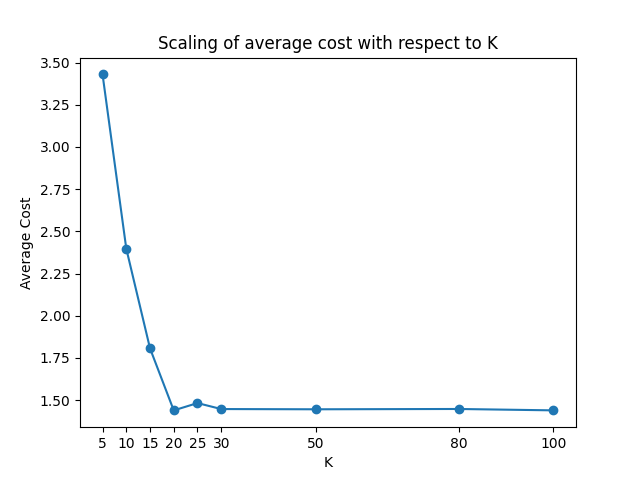
\includegraphics[scale = 0.5]{Figure_1_2.png}
    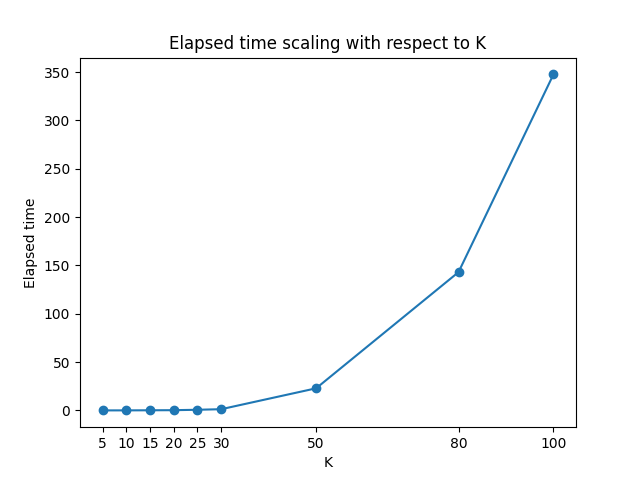
\includegraphics[scale = 0.5]{Figure_1_3.png}
    \caption{Scaling of average cost and elapsed time with respect to K for $\alpha = 0.8, u_{min} = 0.2, q=0.2, C=0.2K$}
\end{figure}
The observed results align closely with our initial expectations. As anticipated,
 we witnessed a decrease in the average cost and an increase in the elapsed timeas the number of states (K) increased. However it remains unclear whether the average cost at which our algorithm converged ($\approx 1.44$ as shown in the figure above) is optimal or not. 
In an attempt to better understand the results, we proceeded to eliminate any randomness from the environment by setting $\alpha = 1, u_{min} = 0$
\begin{figure}[H]
    \centering
    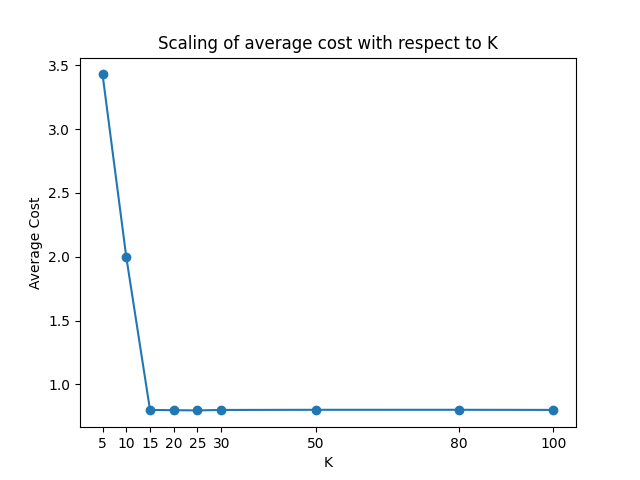
\includegraphics[scale = 0.5]{Figure_21.png}
    
    \caption{Scaling of average cost and elapsed time with respect to K for $\alpha = 1, u_{min} = 0.0, q=0.2,C=0.2K$}
\end{figure}
In Figure 2, we observe that the curve stabilizes at an average cost of approximately 0.8.
 Unlike the result shown in Figure 1, this outcome makes perfect sense. In this case, we consider a user
  who always selects from the recommendation batch. Assuming we have a sufficient number of cached items
   to choose from (large K), the user will be directed 100\% of the times to a cached video, resulting in 
   a total cost of 0. The reason the average cost is 0.8 is because the initial state is chosen randomly, 
   with a 0.8 probability of being uncached and a 0.2 probability of being cached (thus yielding an average cost of 0.8). 
   Essentially 0.8 is the minimum cost that can be achieved, indicating that our algorithm works correclty.

   At this point, we decide to attempt explaining the average cost of $1.44$ in Figure 1 by constructing a formula which calculates the minimum average cost of a session ($E(S)$) given the parameters $\alpha,q$.
Essentially we are trying to come up with a formula that returns the optimal average cost at which our algorithm should converge as $K \rightarrow \infty$.
Eventually, we derived the relationship below, which will be proven in the appendix.
\begin{align*}
    E[S] = 0.8 + 0.8(\frac{1}{q}-1)(1-\alpha)  \tag{1}
\end{align*}
Note that we can completely ignore the $u_{min}$ factor when $K\rightarrow \infty$. This is because, in the case of an infinite number of videos, there will also be an infinite number of cached videos. As a result,
 there will always be at least 2 cached and relevant videos available for recommendation, regardless of the value of $u_{min}$.
    Now if we set $\alpha =0.8$ and $q=0.2$ we get 
    $$E[S] = 0.8 + 0.8\cdot 4\cdot 0.2=1.44$$
    which is the result obtained in Figure 1, proving that our policy iteration algorithm converges optimaly.
    To further confirm the validity of the formula $(1)$ we proceed to plot average cost escalation with respect to i) $\alpha$ ii) $q$ for a relatively large K.
    What we wish to see is a linear decreasing relationship over $\alpha$ and hyperbolic decreasing relationship over $q$, as formula (1) suggests
    \begin{figure}[H]
        \centering
        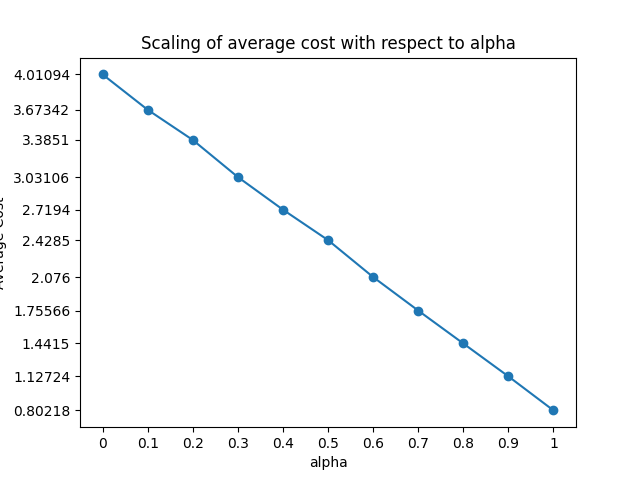
\includegraphics[scale = 0.5]{Figure_31.png}
        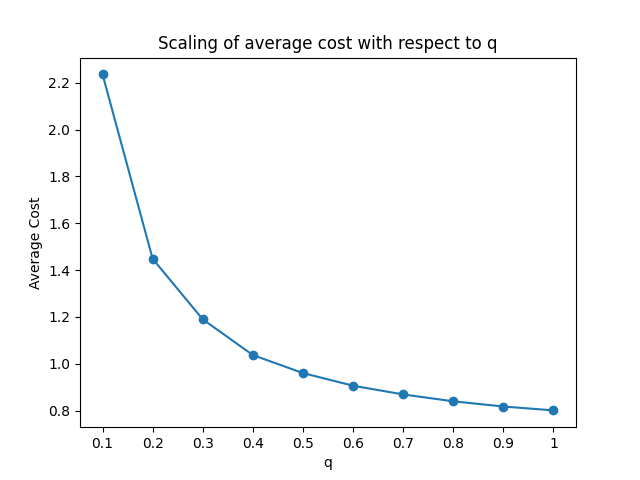
\includegraphics[scale = 0.5]{Figure_32.png}
        \caption{Scaling of average cost w.r.t. $\alpha$ (Left) for $C=0.2K$, $K=30, u_{min} = 0.2, q=0.2$ and w.r.t $q$ (Right) for $K=30, u_{min} = 0.2, \alpha=0.8$}
    \end{figure}
    Indeed, we observe the anticipated results, confirming the validity of our formula. Lastly, we want to examine the escalation of the average cost with respect to $u_{min}$. As previously clarified, if $K \rightarrow \infty$, $u_{min}$ should not have any impact on the average cost. However, for finite values of $K$ (e.g., $K=50$), 
    we expect the average cost to remain unaffected by $u_{min}$ as it is still small, and then start increasing thereafter. Unfortunately, we do not have a formula to predict this escalation as we do for $\alpha$ and $q$.\begin{figure}[H]
        \centering
        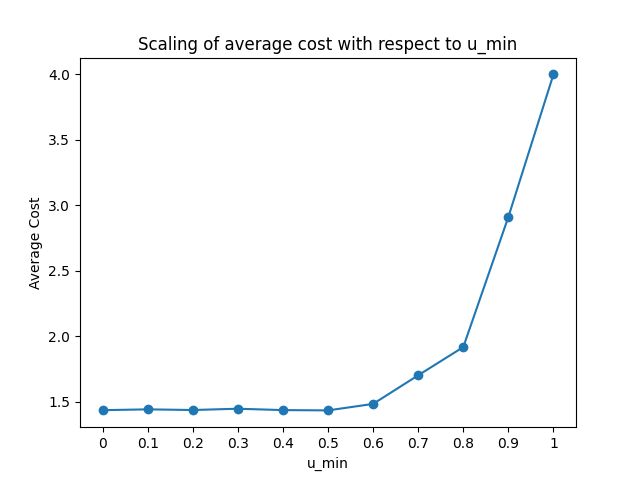
\includegraphics[scale = 0.5]{Figure_33.png}
        \caption{Scaling of average cost w.r.t. $u_min$ for $K=50, \alpha = 0.8, q=0.2$, $C=0.2K$}
    \end{figure}
    \section*{Parameters slelection for Q-Learning}
    \begin{itemize}
        \item The parameter $\epsilon$ determines the exploration-exploitation trade-off in Q-learning.
        Initially, we settled with a constant $\epsilon$ and we observed that for larger values of $K$, a larger $\epsilon$ was needed to ensure sufficient exploration and prevent the algorithm from getting stuck in suboptimal policies. We also tried a decreasing over $t$, $\epsilon$ which does work, but still encouters the same issue as before.
        To address this, we adopted the same epsilon-greedy for bandits formula $\epsilon = \frac{1}{t^\frac{1}{3}}(\#actions \log(t))^\frac{1}{3}$.
        \item Regarding the learning rate parameter, our goal is to strike a balance between learning speed and stability. A learning rate that is too small may lead to slow convergence, while a learning rate that is too large can result in high fluctuation around the target.
         Through empirical experiments, we conclude in a learning rate $ = 0.01$
        \item The number of iterations was set to be $2000K$. This value was determined through a trial and error process, and it was found to be sufficient for achieving optimal convergence. Therefore, the scalability of the algorithm with respect to K is $O(K)$, indicating a linear relationship between the number of iterations and the value of K.
    \end{itemize}
        \section*{Experimental Evaluation of Q-Learning}
        In our experiments, we plotted two key metrics to evaluate the performance of the Q-learning algorithm in comparison to the policy iteration algorithm.
        The first plot represents the average cost on the y-axis against the number of videos, denoted as K, on the x-axis. The second plot illustrates the elapsed 
        time of the algorithm on the y-axis, also against the number of videos K on the x-axis.
        \begin{figure}[H]
            \centering
            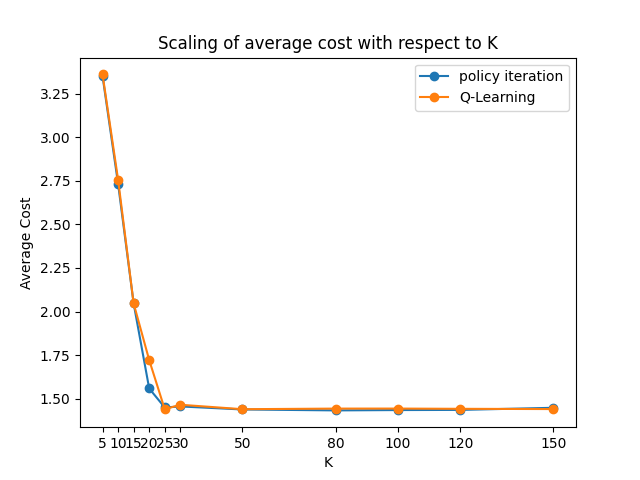
\includegraphics[scale = 0.5]{Figure_69.png}
            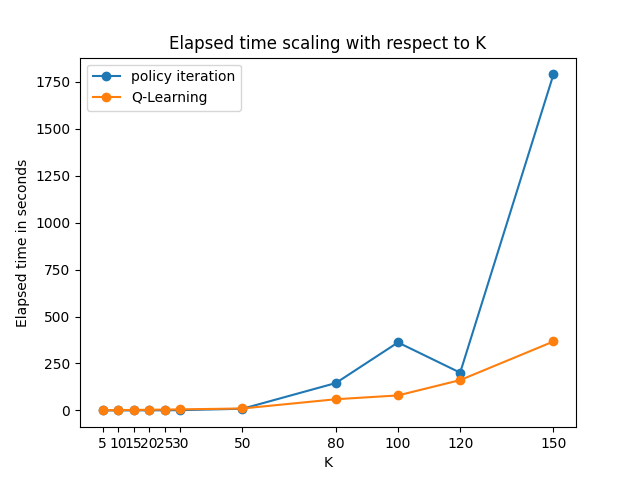
\includegraphics[scale = 0.5]{Figure_70.png}
            \caption{Scaling of average cost and elapsed time with respect to K for $\alpha = 0.8, u_{min} = 0.2, q=0.2, C=0.2K$ for policy iteration and Q-Learning}
        \end{figure}
        Upon analyzing the plots, we made several key observations. Firstly, we observed that the Q-learning algorithm line coincides with policy iteration line, indicating their similar performance in terms of average cost.
        This provides strong evidence that Q-Learning learns the optimal policy  as effectively as policy iteration . It is important to note that these two algorithms may not find the exact same policies since there can be multiple equivalent policies. However, both algorithms converge to a policy that minimizes the cost.

        Regarding the elapsed time of the algorithms, we observed that Q-Learning is faster than policy iteration, as expected. This is because Q-Learning scales in $O(K)$, whereas policy iteration scales in $O(K^2)$. We also observed that for $K=150$, policy iteration requires half an hour to converge. On the other hand,
         the corresponding breaking point for Q-Learning was found to be $K=200$.
        \section*{Appendix}
        \subsection*{Toy example}
        
    $$U=\begin{pmatrix}
        0&0.8&0.3&0.6\\
        0.8&0&0.7&0.2\\
        0.3&0.1&0&0.2\\
        0.6&0.4&0.2&0\\
    \end{pmatrix}$$
    $$Cost = \left[1,0,1,0\right],\;\;\alpha = 0.8,\;\;q=0.2,\;\;u_{min} = 0.2$$
    The optimal policy given by our algorithm is:
    $$\pi[0] = (1,3),\;\pi[1] = (0,3),\;\pi[2] = (0,3),\;\pi[3] = (0,1)$$
    
        \subsection*{Proof of formula (1)}
        Initially, we will have to calculate the average cost of
        watching a video given the parameter $\alpha$. Let $X\in \{0,1\}$ be the cost of video. then we have
          $$E[X] = 0P(C)+1P(U)=P(U)$$
          where $P(C)$ is the probability of the video being cached and $P(U)$ the probability of the video being uncached. 
          $$P(U) = P(U|A)P(A)+ P(U|\bar{A})P(\bar{A})$$
          Here, $A$ denotes the event of choosing a video from the recommendation batch, so $P(A) =\alpha$. Since we are intersted only on large $K$, we can make the assumption that no item in the recommendations batch is uncached, thus choosing an uncached video from the recommended is impossible
          ($P(U|A) = 0$). On the other had choosing an uncached video out of all videos has probability 0.8.
          $$P(U) = \cancelto{0}{P(U|A)}P(A)+ P(U|\bar{A})P(\bar{A}) = 0.8(1-\alpha)$$
          
          In order to calculate the average cost of a session, it may be tempting to take the product of the average number of 
          videos during a session with the average cost of a video ($E[X]$). However, due to the initial state being chosen
           randomly with an average cost of 0.8, we need to add it separately. If we denote the average number of videos in
            a session as $E[n] = 1/q$, the average cost of the session can be calculated as follows:
           \begin{align*}
               E[S] = 0.8 + (E[n]-1)E[X] = 0.8 + 0.8(\frac{1}{q}-1)(1-\alpha)  
           \end{align*}
           Note that the constant 0.8 actually corresponds to $1-\frac{C}{K}$ for $C=0.2K$. Therefore, the generalization of the formula for any value of $C$ would be:

\begin{align*}
E[S] = \left(1-\frac{C}{K}\right) + \left(1-\frac{C}{K}\right)(\frac{1}{q}-1)(1-\alpha)
\end{align*}
If we were to plot $E[S]$ over $C$, it would exhibit a linear decreasing relationship
        \end{document} 